\section{Ableitung}
  \subsection{Differenzenquotient/Differentialquotient}
  \begin{definition}
    Die Änderung einer Funktion heißt Differenzenquotient:
    \begin{equation}
      \frac{f(x_n)-f()x_0)}{x_n - x_o}
    \end{equation}
  \end{definition}
  \begin{definition}
    Gegeben sei $f: I\rightarrow \R$ und ein Punkt $x_o \in I$. Die Funktion $f$ heißt differenzierbar in $x_0$, falls der Grenzwert
    \begin{equation}
      \lim_{x\rightarrow x_0} \frac{f(x) - f(x_0)}{x - x_0} = \lim_{h \rightarrow 0} \frac{f(x_0 + h) - f(x_0)}{h}
    \end{equation}
    existiert. Der Grenzwert heißt der Differentialquotient bzw. die Ableitung von $f$ in $x_0$ und wird mit $f'(x_0)$ bzw. $\diff{f}{x}(x_0)$ bezeichnet.
  \end{definition}
  \begin{bem}
    Die Ableitung $f'(x_0)$ gibt die Steigung der Tangente an $f$ in $x_0$ an. Die Tangentengleichung ist:
    \begin{equation}
      l(x) = f(x_0) + f'(x_0)(x-x_0)
    \end{equation}
    Es gilt:
    \begin{align}
      &l(x_0) = f(x_0) + f'(x_0)(x_0 - x_0) = f(x_0) \\
      und\nonumber \\
      &l'(x_0) = f'(x_0)
    \end{align}
    d.h. der Funktionswert und die Ableitung von $f$ und $l$ stimmen in $x_0$ überein.
  \end{bem}
  \subsection{Stetigkeit}
  \begin{definition}
    Eine Funktion $f$ heißt stetig in $x_0$, falls 
    \begin{equation}
      \lim_{x \rightarrow x_0} f(x) = f(x_0)
    \end{equation}
  \end{definition}
  \begin{satz}
    Jede in $x_0$ differenztierbare Funktion ist auch stetig in $x_0$  
  \end{satz}
  \begin{bem}
    Merkregel:\newline
    Stetig: $f$ kann durchgezeichnet werden.\newline
    Diffbar: $f$ hat keinen Knick
  \end{bem}
  Beispiel:\newline
  $f(x) = |x|$ ist in $x_0 = 0$ stetig aber nicht diffbar.
  \begin{bem}
    Bezeichnungen:
    \begin{itemize}
      \item $C^0$: Menge aller stetigen Funktionen
      \item $C^1$: Menge aller diffbaren Funktionen mit $f,f'$ stetig
      \item $C^n$: Menge der n-mal stetig diffbaren Funktionen, d.h. $f, f', \dots, f^{(n)}$
      \item $C^{\infty}$: Menge aller unendlich oft stetig diffbaren Funktionen
    \end{itemize}
  \end{bem}
  \subsection{Wichtige Ableitungen}
  \begin{equation}
    f(x) = x^n \rightarrow f'(x) = nx^{n-1}
  \end{equation}
  \begin{equation}
    f(x) = e^x \Rightarrow f'(x) = e^x
  \end{equation}
  \begin{equation}
    f(x) = ln(x) \Rightarrow f'(x) = \frac{1}{x}
  \end{equation}
  \begin{equation}
    f(x) = arctan(x) \Rightarrow f'(x) = \frac{1}{(tan(y))'}
  \end{equation}
  \begin{equation}
    f(x) = arcsin(x) \Rightarrow f'(x) = \frac{1}{(sin(y))'}
  \end{equation}

  \subsection{Ableitungsregeln}
  \begin{satz} Produkt-/Quotientenregel\newline
    \vspace{-0.5cm}
    \begin{itemize}
      \item[a) ] Seien $\alpha ,\beta \in \R$, dann gilt
        \begin{equation}
          (\alpha f + \beta g)'(x) = \alpha f'(x) + \beta g'(x) \text{\colBlue{(Linearität der Ableitung)}}
        \end{equation}
      \item[b) ] ~\\[-28pt]
        \begin{equation}
          (fg)'(x) = f'(x)\cdot g(x)+f(x) \cdot g'(x)
        \end{equation}
      \item[c) ] ~\\[-28pt]
        \begin{equation}
          (\frac{f}{g})'(x) = \frac{f'(x)g(x)-g'(x)f(x)}{\big(g(x)\big)^2}
        \end{equation}
    \end{itemize}
  \end{satz}
  \begin{satz} Kettenregel\newline
    \vspace{-0.5cm}
    \begin{itemize}
      \item[a) ]Es gilt:
      \begin{equation}
        (g \circ f)'(x) = g' \big(f(x)\big) \cdot f'(x)
      \end{equation}
      \item[b) ] Es sei $f: [a,b] \rightarrow \R$ streng monoton wachsend mit $f'(x_0) \neq 0$ und diffbar. Dann existiert die Umkehrfunktion $f^{-1}:[f(a), f(b)] \rightarrow \R$ und besitzt die Ableitung
      \begin{equation}
        \left( f^{-1}\right)'(y_0) = \frac{1}{f'(x_0)}
      \end{equation}
      mit $y_0 = f(x_0)$.
    \end{itemize}
  \end{satz}
  \newpage
  
  \subsection{Mittelwertsätze}  
  \begin{definition}
    Es sei $f:(a,b)\rightarrow \R$ und $x_0 \in (a,b)$.
    \begin{itemize}
      \item[a) ]$f(x)$ hat in $x_0$ ein lokales Maximum, falls es ein $\varepsilon > 0$ gibt mit $f(x) \leq f(x_0)$ für alle $x \in (a,b)$ mit $(x-x-0) < \varepsilon$.
      \item[b) ] Analog für lokales Minimum. 
    \end{itemize}
  \end{definition}
  \vspace{-0.5cm}
	  \begin{figure}[H]
	  \centering
	  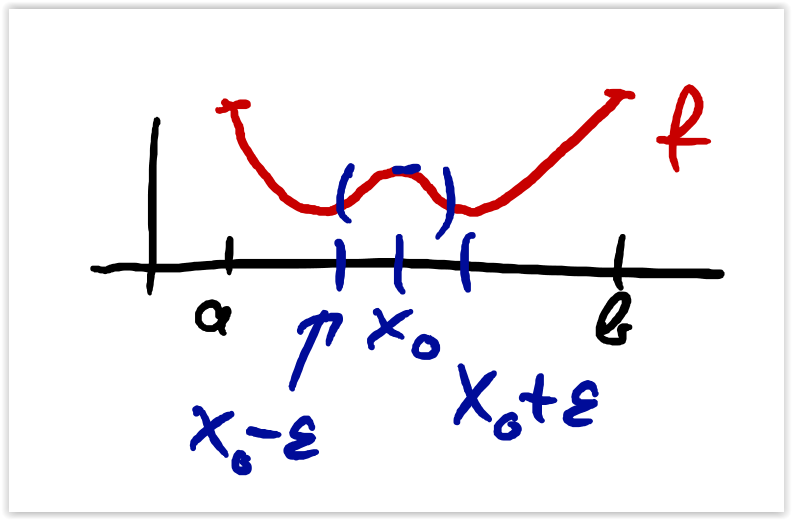
\includegraphics[width=0.3\textwidth]{./img/mws_def.png}
	  \caption{Lokales Minimum/Maximum\protect\cite{HM12}}
	  \label{fig:mws_min_max}
	\end{figure}
  \begin{satz}
    Besitzt eine stetig diffbare Funktion $f: (a,b) \rightarrow \R$ in einer Stelle $x_0 \in (a,b)$ ein lokales Maximum oder Minimum, so gilt notwendigerweise $f'(x_0) = 0$.
  \end{satz}
  \begin{satz}
    Seien $f,g:[a,b] \rightarrow \R$ stetig und auf $(a,b)$ diffbar mit $g'(x) > 0$ bzw. $g'(x) <0$ jeweils für alöle $x \in (a,b)$. 
    \begin{itemize}
      \item[a) ] \textbf{Satz von Rolle:} Gilt $f(a) = f(b)$, so existiert ein $\xi \in (a,b)$ mit $f'(\xi) = 0$.
      \item[b) ] \textbf{1. Mittelwertsatz:} Es gibt ein $\xi \in (a,b)$ mit $f'(\xi) = \frac{f(b) - f(a)}{b-a}$.
      \item[c) ] \textbf{2. Mittelwertsatz:} Es gibt ein $\xi \in (a,b)$ mit $\frac{f'(\xi)}{g'(\xi)} = \frac{f(b) - f(a)}{g(b) - g(a)}$.
    \end{itemize}
  \end{satz}
  \begin{figure}[H] 
		\centering
		\begin{minipage}{.5\textwidth}
		  \centering
		  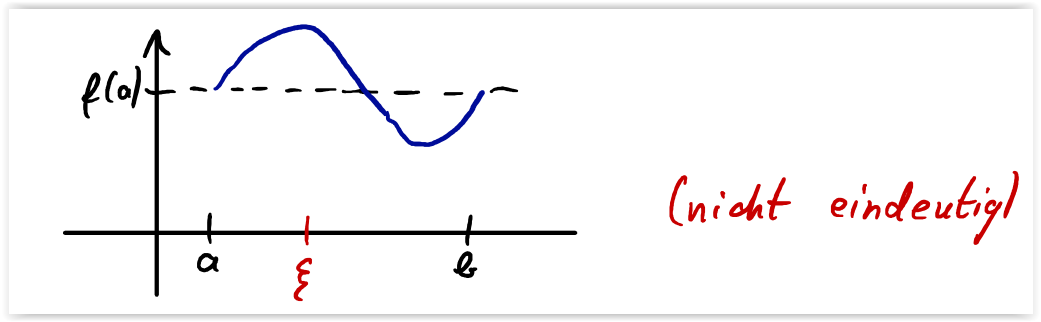
\includegraphics[width=0.8\linewidth]{./img/mws_rolle.png}
		  \caption{Zu a) \protect\cite{HM12}}
		  \label{fig:mws_rolle}
		\end{minipage}%
		\begin{minipage}{.5\textwidth}
		  \centering
		  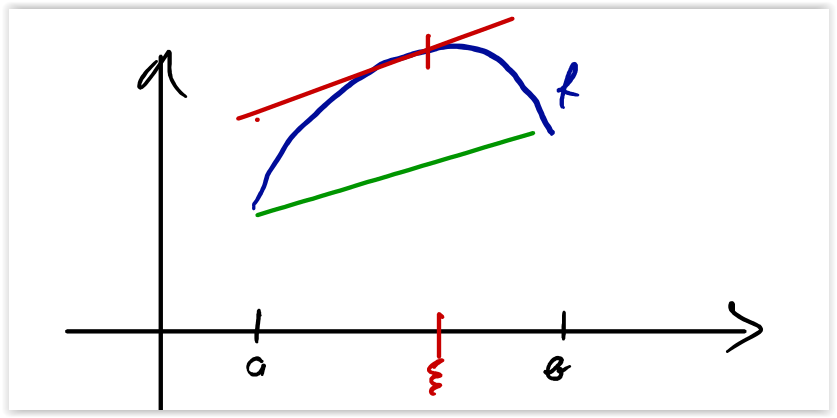
\includegraphics[width=0.8\linewidth]{./img/mws_1.png}
		  \caption{Zu b) \protect\cite{HM12}}
		  \label{fig:funkt_sinh}
		\end{minipage}
  \end{figure}
		
  \subsection{Monotonie}	
  \begin{satz}$\;$ \newline
  \vspace{-0.5cm}
    \begin{itemize}
      \item[a) ] Ist $f:(a,b)\rightarrow \R$ differenzierbar und ist $f:[a,b]\rightarrow \R$ stetig und es gelte $f'(x_0) = 0 \quad \forall x \in (a,b)$, so ist $f$ konstant.
      \item[b) ] 
      \begin{tabular}{l c l} 
        $f'(x) \geq 0 \quad \forall x \in (a,b)$ & $\Leftrightarrow$ & $f$ ist monoton wachsend \\
        $f'(x) > 0 \quad \forall x \in (a,b)$ & $\Rightarrow$ & $f$ ist streng monoton wachsend \\
        $f'(x) \leq 0 \quad \forall x \in (a,b)$ & $\Leftrightarrow$ & $f$ ist monoton fallend \\
        $f'(x) < 0 \quad \forall x \in (a,b)$ & $\Rightarrow$ & $f$ ist streng monoton fallend \\
      \end{tabular}
    \end{itemize}
  \end{satz}	
  
  \subsection{Das Prinzip von l'Hospital}
  \begin{satz}
    Gilt $\lim\limits_{b\rightarrow a} f(b) = 0$, $\lim\limits_{b\rightarrow a} g(b) = 0$ und existiert $\lim\limits_{b\rightarrow a} \frac{f'(b)}{g'(b)}$, so existiert auch $\lim\limits_{b\rightarrow a} \frac{f(b)}{g(b)}$ und er ist gleich $\lim\limits_{b\rightarrow a} \frac{f'(b)}{g'(b)}$. Analog $\lim\limits_{b\rightarrow a} f(b) = \infty$ und $\lim\limits_{b\rightarrow a} g(b) = \infty$.
    \begin{equation}
      \Rightarrow \lim\limits_{b\rightarrow a} f(b) = 0 \land \lim\limits_{b\rightarrow a} g(b) = 0 \land \lim\limits_{b\rightarrow a} \frac{f'(b)}{g'(b)} \Rightarrow \lim\limits_{b\rightarrow a} \frac{f'(b)}{g'(b)} = \lim\limits_{b\rightarrow a} \frac{f(b)}{g(b)}
    \end{equation}
  \end{satz}
  \begin{bem}
    Zur Berechnung muss der Ausdruck gegebenenfalls auf $"\frac{0}{0}"$ zurückgeführt werden. Entspricht zum Beispiel $\frac{f(b)}{g(b)}$ der Form $"\frac{\infty}{\infty}"$ kann durch Umformung zu $\frac{\frac{1}{f(b)}}{\frac{1}{g(b)}}$ l'Hospital angewandt werden.\newline
    Liegt ein Ausdruck in der Form $"\infty \cdot 0"$ wie zum Beispiel $\lim\limits_{x\rightarrow \infty} \underbrace{x}_{\rightarrow \infty} \underbrace{ln\left(\frac{x+1}{x-1}\right)}_{\rightarrow 0 }$ vor, kann durch Umformung zu $\lim\limits_{x\rightarrow \infty} \frac{ln\left(\frac{x+1}{x-1}\right)}{\left(\frac{1}{x}\right)}$ wieder in die Form $"\frac{0}{0}"$ gebracht werden.
  \end{bem}
  \newpage
  
\section{Taylorpolynome}
  \begin{satz}
  Sei $f:I\rightarrow \R$ eine $C{n+1}$ Funktion und sei $x_0 \in I$ und heißt Entwicklungspunkt. Dann ist
  \begin{itemize}
    \item[a) ] das Taylorpolynom n-ten Grades zum Entwicklungspunkt $x_0$ gegebn durch
    \begin{equation}
    T_n(f, x, x^*) = \sum\limits_{k= 0}^n \frac{f^{(k)}(x^*)}{k!} (x-x^*)^k
    \end{equation}
    und stimmt mit $f$ in $x_0$ bis zur n-ten Ableitung überein.
    \item[b) ] Der Fehler 
    \begin{equation}
      R_n(x,x_0) = f(x) - T_n(x,x_0)
    \end{equation}
    ist gegeben durch die Restgliedformel nach Lagrange
    \begin{equation}
      R_n(x,x_0) = \frac{f^{(n+1)}(\xi)}{(n+1)!}(x-x_0)^{n+1}
    \end{equation}
    wobei $\xi = x_0 + \Theta (x-x_0)$ mit $\Theta \in (0,1)$, d.h. $\xi$ ist eine Zahl zwischen $x$ und $x_0$. Es gilt dann
    \begin{equation}
      \big|R_n(x,x_0)\big| = \frac{\sup\limits_{\xi \in (x_0,x)} \left|f^{(n+1)}(\xi)\right|}{(n+1)!}|x-x_0|^{(n+1)}
    \end{equation}
  \end{itemize}
  \end{satz}  
\newpage
